%!TEX root = ../thesis.tex

\cleardoublepage
\chapter{Background}
\label{cha:background}


This chapter provides background information on and explanations of the functionality and purpose of some of the technologies and concepts related to this thesis.  To begin, the history of distributed computing and containerization are discussed in sections \ref{sec:dist-computing} and \ref{sec:containers} before moving on to a discussion of their current usage in scientific workflows in \ref{sec:workflows}. After that the workflow manager used in this thesis, nextflow, is introduced in section \ref{sec:nextflow}. Finally, in \ref{sec:rl} reinforcement learning is touched upon and its functionality as well as the benefits it could bring to the problem at hand are briefly discussed.

%%=========================================
\section{Distributed Systems, Batch Processing and Cloud Computing}
\label{sec:dist-computing}

Within the context of this thesis and scientific workflows it makes sense to discuss some of the ways in which tasks or jobs that have long run times and require large amounts of resources can be carried out. In general for a given user who needs to execute a workflow there are really only four options namely 1) running it on their personal computer, which quickly becomes infeasible for large and difficult tasks, 2) using a cloud computing service, 3) using hardware with significantly more resources or 4) using a distributed system such as a cluster or grid. Of these four options number 1 and 3 obviously need no special explanation but cloud computing and distributed systems deserve to be briefly defined.

While there is a lot of debate to be had about what precisely constitutes a distributed system the article “Programming Languages for Distributed Systems” by Bal, Steiner and Tanenbaum generally defines a distributed system as one in which “multiple autonomous processors do not share memory but cooperate by sending messages over a communications network” \cite{Tanenbaum} . Building on this definition, for this thesis the term distributed computing is considered to be the performance of a single computational task across multiple distinct machines. Usually this task is quite large or difficult, or is an aggregate of various smaller tasks but the core idea remains the same. Within the term ‘distributed computational system’ many distinctions can be made regarding the exact architecture of the distributed system but the two which are specifically relevant to this thesis are only grids and the types of clusters typically used at universities.  One of the possible uses for distributed systems is for parallel high-performance applications because of the vast resources available in the system.

TODO: batch processing?

Unlike the definition of what constitutes a distributed system, a cloud computing service is quite easy to define and can be considered any service which provides on-demand access to a flexible amount of computing resources. These services must be paid for of course and are heavily reliant on virtualisation. Cloud computing provides a configurable amount of computing resources so that users only pay for what they need. A given user or group of users no longer need their own computing resources but can instead purchase them from cloud computing providers which relieves them of the burden of maintaining and managing such systems as well. 

For scientific workflows both distributed systems and cloud computing services represent excellent deployment architectures for increased performance due to the increased resources available in such systems.

%%=========================================
\section{Containerization}
\label{sec:containers}

Virtualization has existed for a long time however the overhead of running a virtual machine is often not worth the advantages it provides. Particularly for reproducible software development the most important qualities of the host machine may not even be the architecture but rather the interactions with the operating system and its filesystem. Software containers are a type of virtualisation which do not virtualise the architecture of the host machine but instead use namespaces and control groups to virtualise the operating system, network, filesystem and all of the other peripheral components a program interacts with. This enables containers to isolate processes from the host machine and also from each other. Specifically for the deployment of applications and software this provides a humongous advantage. With containers it is possible, for example, to run two different versions of the same software on the same machine or even to run two versions of the same software but with two different configurations in parallel to each other. In addition to this the software will not know anything of the other version of itself running in parallel. Most importantly, in both of these cases the behaviour of the programs in the containers should always be the same. This is because a software container provides a sanitized version of the host system where there is no danger of other users or processes interacting with the filesystem or using the devices made available by the operating system.

Beyond the benefits for co-locating services on the same machine without minimal danger of interference, containerization also simplifies the process of deploying software to a new machine. If a given machine supports the running of containers then all that is needed to deploy one's software on that machine is an image or container of the software. One of the most popular containerization softwares is Docker. Their philosophy is ``build once, deploy anywhere'', and many cloud computing services only need to be provided an image of a container and they can instantly deploy that service. This simplifies software deployment for the software developers as well as the management of the machines on which they run. In addition to this it also becomes easy to scale applications up or down. Adding more resources to a container or starting a new machine running the same application becomes a trivial process. Lastly, for managers of cloud computing centers the additional layer of virtualization offered by containers enables them to move containers and applications between different machines. 

This is particularly useful for scientific workflows because by using containers the tasks that make up a workflow can all be reliably reproduced on various different execution platforms. 

%%=========================================
\section{Scientific Workflows}
\label{sec:workflows}

With the increased use of simulations and digital sensors the importance of digital data in the sciences continues to rise\cite{ScientificWorkflows}. In addition to this, the computational tasks being performed on this data are more complex and must process larger data volumes than ever before. This has led to unprecedented computing power requirements in the sciences. Indeed much of the effort of scientists is now invested in the analysing and processing of the data rather than the gathering of the data and software costs have come to dominate capital expenditures for many large-scale experiments \cite{Gray}. Some of the scientific fields which have particularly large computational needs are Biology, Astronomy, and Seismology \cite{ScientificWorkflows}. 

To handle so much data it is usually processed in a sequence of small individual steps or tasks, often using command-line tools, in a sophisticated structure of dependencies and pipelines. Since these tasks may work on the same data or a version of that data that has been processed by another task there are of course temporal and logical dependencies between the tasks. Managing these complex interdependent structures can be quite difficult and has given rise to the concept of workflows, which are meant to simplify modelling all of the the tasks and workflow managers which aid in carrying them out. 

Workflows can be modelled in many different ways, ranging simple scripting languages through to graphs and mathematical models \cite{Shields}. At their core, workflows consist of four simple components: the inputs, the tasks, the dependencies between tasks, and the outputs. This can easily be modelled as a graph with vertices to represent tasks and edges to represent dependencies. An example of this can be seen in \ref{fig:dag}. 

\begin{figure}[ht]
    \centering
        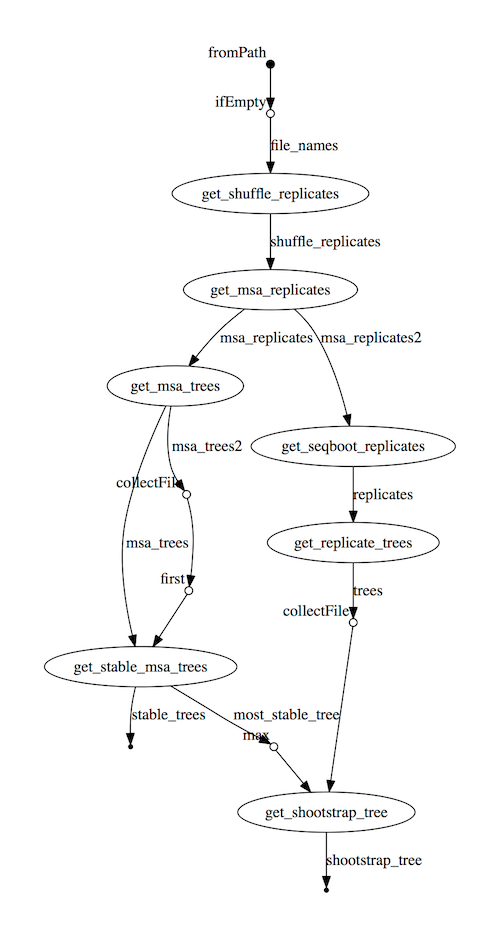
\includegraphics[width=0.6\textwidth,height=0.9\textheight]{fig/dag.png}
        \caption{nf-core/shootstrap Workflow Represented as a Digraph \cite{dag}}
        \label{fig:dag}
\end{figure}




%%=========================================
\section{Workflow Management Systems}
\label{sec:management}



%%=========================================
\section{Nextflow}
\label{sec:nextflow}

%%=========================================
\section{Reinforcement Learning}
\label{sec:rl}

Popularized in the seminal book (TODO: cite!) by Sutton and Barto, reinforcement learning presents a framework for an agent to learn the optimal policy for achieving a given goal in an uncertain environment by interacting with the problem and the environment. And most importantly it is able to adjust this policy ``on the go'', meaning it can both learn a new policy if the challenge or the environment changes and that it can be deployed immediately without any training and it will improve as it gains experience. In this context the agent's goal is always set by a reward function. Using reinforcement learning, the agent learns to maximize this function and thus, hopefully, to achieve the goal of its designers. 

Central to reinforcement learning are the policies and how best to evaluate them. In order to achieve its goal an agent needs to develop a policy that maximizes its reward, then as the agent encounters similar situations it simply follows the policy it has learned. To evaluate a policy it must be compared to the ideal version of itself. For any given problem and its reward function there exists at least one policy which maximizes the reward. At its core, reinforcement learning aims to enable the agent to continuously refine its current policy so that it approaches the optimal policy. 

Even more important than the concept of policies is the idea of exploration vs. exploitation. Since the agent initially knows nothing about its environment it must attempt  to learn about its environment through exploration. By trying different choices and receiving different rewards the agent can construct a policy that always makes the right choice. But in order to know what the right choice is the bandit must also make the wrong choice so that it can learn not to make it again. Trying different things is the ''exploration'' and using the knowledge gained from this to make the right choice is the ``exploitation''. An agent cannot simultaneously explore and exploit. This is dichotomy is at the core of reinforcement learning. The agent must always make the choice between exploring more to potentially discover an even better policy and eventually yield even better rewards, and using its current policy to increase its rewards. 

In this thesis two specific types of reinforcement learning are considered. First are gradient bandits. The term ``Bandits'' is a framework for solving problems in which an agent repeatedly returns to an unchanging situation in which there are several choices, each of which lead to unknown results. The analogy used by Sutton and Barto is of a room with several levers with unknown effects (the pulling of a certain lever may also be called the action). From the bandit's perspective pulling any of the levers yields a certain reward and it is the bandit's task to find a policy which yields the maximum reward from the pulling of certain levers. Applying this to the case of nextflow and the sizing of tasks one can consider the levers, or the choice, as the resource configuration. The bandit is asked repeatedly to allocate a certain amount of resources for a task (equivalent to pulling one of the levers) and must find the best policy for this (where the policy could be minimizing runtime or maximizing resource usage). Gradient bandits solve this problem of finding the best policy by using the gradient of the reward function to learn a preference for each of the levers. Using gradient ascent the bandits take small steps in the direction of a the ideal preference for each lever which would maximizes the reward. Mathematically speaking this is done through stochastic gradient ascent, for which the formula is : TODO use equation $H_{t+1} = H_t(a) + \alpha \frac{ \delta E[R_t] }  {\delta H_t(a)}$. This formula aims to increment the preference proportional to the increment's effect on performance. These preferences influence the probability of choosing a given action. Crucially, after choosing an action and receiving the reward the preferences for all of the actions are updated to try and follow the gradient of the reward. In practice however the expected reward for each action is not known- if it were known the problem would be trivial and the agent could be configured to always pick the maximizing action. Instead the expected reward function and its gradient must be approximated over time. This leads to the formula for updating the preferences proposed by Sutton and Barto. For a preference $H_{t+1}$ after taking action $A_t$ and receiving reward $R_t$ its preference is updated as follows TODO use begin equation: $H_{t+1}(A_t) = H_t(A_t) + \alpha (R_t - \hat{R}) (1 - \pi_t(A_t))$ and $H_{t+1}(a_t) = H_t(a_t) - \alpha (R_t - \hat{R})\pi_t(a_t)$ for the preferences for each action $a_t != A_t$ , where $\hat{R}$ is the average of all the rewards so far. It can be proven that this formula eventually approximates the formula for gradient ascent.

TODO: states and Q or TD learning
